%----------------------------------------------------------------------------------------
% DE COVARIANTIEMATRIX. Alle opgaven zijn eigen werk; alle gegevens zijn verzonnen.
%
% Opbouw: Probleem, Start, leerstof (theorie, werkwijze of uitleg, voorbeeld, korte oefening), en op een
% nieuwe pagina de Opdrachten (door elkaar, stijgende moeilijkheid), Koppel en Test jezelf.
% Labels van dit hoofdstuk beginnen met h2-.
%----------------------------------------------------------------------------------------

\mychapter{2}{De covariantiematrix}

\begin{probleem}
Een school geeft in het zesde jaar drie proefexamens: wiskunde ($W$), fysica ($F$) en Nederlands ($N$), elk op 40. Het verslag aan de klassenraad vat de resultaten samen met de standaardafwijkingen $s_W = 4$, $s_F = 3$ en $s_N = 2$, en de covarianties
\[ s_{WF} = 6, \qquad s_{WN} = 4, \qquad s_{FN} = 3 . \]
Voor de rapporten telt de school de drie scores op: $T = W + F + N$. Hoe groot is de standaardafwijking van het totaal? Is het $4 + 3 + 2 = 9$, of $\sqrt{4^2 + 3^2 + 2^2} \approx 5{,}4$, of nog iets anders? En hoe sterk spreidt het verschil $W - F$ tussen wiskunde en fysica? De punten per leerling staan niet in het verslag.
\end{probleem}

\lkr{Leerplan Complementair (III-WiCo-d): LPD 53 (de definitie, eigenschappen en beperkingen van de covariantiematrix van een steekproef uit een multivariate verdeling toelichten), met de wenk over de berekening met ICT. Voorkennis uit pakket 4: Matrices (product, getransponeerde, symmetrische matrix, determinant, inverse, homogene stelsels), Statistiek (variantie met $n - 1$, steekproef en populatie) en hoofdstuk 1 (covariantie, correlatie). De regel $(AB)\tr = B\tr A\tr$ staat niet in Matrices en wordt hier bewezen. Extra: de correlatiematrix, de covariantie van twee lineaire combinaties en de portefeuille als toepassing. Met ICT: in Python \texttt{numpy.cov(X, rowvar=False)} (deelt door $n - 1$), in een rekenblad een tabel met \texttt{COVARIANCE.S} per paar; GeoGebra heeft \texttt{Covariance}, maar deelt volgens de handleiding door $n$: controleer dat met een klein voorbeeld voor je het in de klas gebruikt. De TI-84 rekent met matrices (\texttt{[A]\textasciicircum T*[A]/(n-1)} met een gecentreerde matrix in \texttt{[A]}).}

In hoofdstuk 1 keken we naar twee variabelen tegelijk. Maar bij een leerling, een patiënt of een wagen meet je er meestal veel meer: punten voor elk vak, bloeddruk, cholesterol en gewicht, verbruik, vermogen en massa. Elke twee variabelen hebben een covariantie. In dit hoofdstuk zet je al die getallen in één matrix, de \textit{covariantiematrix}. Dan blijkt matrixrekenen precies te doen wat je nodig hebt: de spreiding van een totaal of een gewogen gemiddelde volgt uit één product van matrices. Je leert ook welke eigenschappen elke covariantiematrix heeft, en wat ze niet kan. Op het einde bereken je de standaardafwijking van het totaal van de drie proefexamens.

\begin{oefeningen}[Start]
\oef{h2-start-1}

\needspace{12\baselineskip}
\oef{h2-verken}
\end{oefeningen}

\lkr{De Verken laat leerlingen de formule $s_{x+y}^2 = s_x^2 + s_y^2 + 2s_{xy}$ zelf vinden met getallen. Wie opdracht 15 van hoofdstuk 1 maakte, kent ze al: laat die leerlingen dan meteen het geval $x - y$ doen.}

%========================================================================================
\section{Meer dan twee variabelen}

\subsection{De gegevensmatrix}

Hoe noteer je gegevens met meer variabelen? Als tabel, met een rij per individu en een kolom per variabele. Voor het rekenen is die tabel een matrix.

\begin{theorie}
Meet je $p$ variabelen bij $n$ individuen, dan is de \textbf{\textcolor{accent}{gegevensmatrix}} $X$ de $n \times p$-matrix met in rij $i$ de metingen van individu $i$: het element $\formule{x_{ij}}$ is de waarde van variabele $j$ bij individu $i$.

De \textbf{\textcolor{accent}{gemiddeldevector}} is de rij $\formule{\overline{\vec x} = (\xbar_1, \xbar_2, \ldots, \xbar_p)}$ met de gemiddelden van de kolommen.

De \textbf{\textcolor{accent}{gecentreerde gegevensmatrix}} $X_c$ ontstaat als je van elke kolom haar gemiddelde aftrekt: $\formule{(X_c)_{ij} = x_{ij} - \xbar_j}$.
\end{theorie}

Elke rij van $X$ is een punt in $\R^p$: bij twee variabelen een punt van het spreidingsdiagram, bij drie een punt in de ruimte. De gemiddeldevector is het gemiddelde punt, het \textit{centrum} van de wolk. Centreren schuift de wolk zo dat het centrum in de oorsprong ligt. De kolommen van $X_c$ zijn de vectoren van afwijkingen uit hoofdstuk 1.

\voorbeeld{}{Vijf leerlingen hebben voor wiskunde, fysica en Nederlands de punten in de tabel. Schrijf de gegevensmatrix, de gemiddeldevector en de gecentreerde gegevensmatrix.

\smallskip
\drietabel[$W$][$F$][$N$]{5}{8 & 10 & 12 & 14 & 16}{10 & 12 & 14 & 13 & 16}{15 & 12 & 16 & 12 & 15}\label{vb:h2-gegevens}}{%
\uitleg{De tabel staat met de leerlingen in de kolommen. In de gegevensmatrix moeten de leerlingen in de rijen staan: we kantelen de tabel.}
\begin{stappenbreed}
X = \um{rrr}{8 & 10 & 15 \\ 10 & 12 & 12 \\ 12 & 14 & 16 \\ 14 & 13 & 12 \\ 16 & 16 & 15} \qquad \overline{\vec x} = (12,\ 13,\ 14) & Een rij per leerling, een kolom per vak. De gemiddelden van de kolommen. \\[10ex]
X_c = \um{rrr}{-4 & -3 & 1 \\ -2 & -1 & -2 \\ 0 & 1 & 2 \\ 2 & 0 & -2 \\ 4 & 3 & 1} & Van kolom 1 trekken we 12 af, van kolom 2 trekken we 13 af, van kolom 3 trekken we 14 af.
\end{stappenbreed}
Elke kolom van $X_c$ heeft som 0: dat geldt voor elke gecentreerde matrix.}

\begin{oefeningen}
\needspace{9\baselineskip}
\oef{h2-gegevens}
\end{oefeningen}

\subsection{De covariantiematrix}

Bij drie variabelen zijn er drie varianties en drie covarianties: $s_{WF}$, $s_{WN}$ en $s_{FN}$. Hoe zet je ze overzichtelijk bij elkaar? In een vierkante tabel, met de variabelen in de rijen en in de kolommen. Op de plaats $(j, k)$ staat de covariantie van variabele $j$ en variabele $k$, en op de diagonaal de covariantie van een variabele met zichzelf: de variantie.

\begin{theorie}
De \textbf{\textcolor{accent}{covariantiematrix}} van een steekproef met $p$ variabelen is de $p \times p$-matrix $S$ met

\vspace{1mm}
\qquad $\formule{s_{jk} = \frac{1}{n - 1}\som (x_{ij} - \xbar_j)(x_{ik} - \xbar_k)}$

\vspace{1mm}
de covariantie van variabele $j$ en variabele $k$. Op de diagonaal staan de varianties $\formule{s_{jj} = s_j^2}$.
\end{theorie}

\naast{\begin{minipage}{9.4cm}
Rechts zie je wat de matrix samenvat voor de vijf leerlingen van voorbeeld \ref{vb:h2-gegevens}. Op de plaats van elke covariantie staat het spreidingsdiagram van die twee vakken. Wiskunde en fysica stijgen samen ($s_{WF} > 0$), wiskunde en Nederlands hebben geen stijgende of dalende tendens ($s_{WN} = 0$). Onder de diagonaal staan dezelfde diagrammen, gespiegeld: daarom laten we ze weg. De matrix is dus symmetrisch, daar komen we op terug.

Hoe bereken je alle elementen tegelijk? De som in de definitie is een rij maal een kolom: kolom $j$ van $X_c$, liggend geschreven, maal kolom $k$ van $X_c$. Dat is het element $(j, k)$ van het product $X_c\tr X_c$.
\end{minipage}}{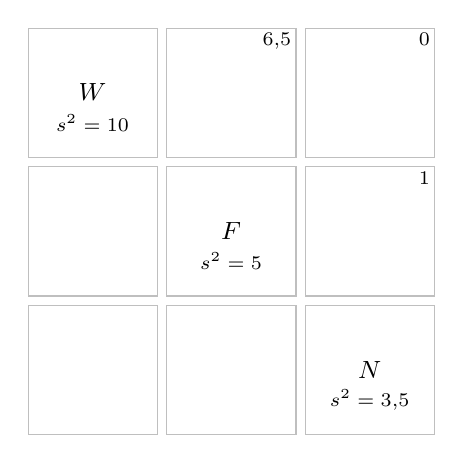
\begin{tikzpicture}[x=.8cm,y=.8cm,font=\scriptsize]
  \foreach \i in {0,1,2}{\foreach \j in {0,1,2}{\draw[black!25] (2.2*\j,-2.2*\i) rectangle ++(2.05,-2.05);}}
  \node[font=\small] at (1.02,-1.02) {$W$};
  \node[font=\small] at (3.22,-3.22) {$F$};
  \node[font=\small] at (5.42,-5.42) {$N$};
  \node at (1.02,-1.5) {$s^2 = 10$};
  \node at (3.22,-3.7) {$s^2 = 5$};
  \node at (5.42,-5.9) {$s^2 = 3{,}5$};
  \begin{scope}[shift={(2.2,-2.05)}]\punten[inkt]{(0.39,0.34) (0.86,0.72) (1.34,1.10) (1.10,1.48) (1.81,1.86)}\end{scope}
  \begin{scope}[shift={(4.4,-2.05)}]\punten[inkt]{(1.42,0.34) (0.47,0.72) (1.73,1.10) (0.47,1.48) (1.42,1.86)}\end{scope}
  \begin{scope}[shift={(4.4,-4.25)}]\punten[inkt]{(1.42,0.39) (0.47,0.86) (1.73,1.34) (0.47,1.10) (1.42,1.81)}\end{scope}
  \node[anchor=north east,inner sep=1.5pt] at (4.25,0) {$6{,}5$};
  \node[anchor=north east,inner sep=1.5pt] at (6.45,0) {$0$};
  \node[anchor=north east,inner sep=1.5pt] at (6.45,-2.2) {$1$};
\end{tikzpicture}}

\begin{theorie}
\begin{stelling}{De covariantiematrix als product}
\qquad $\formule{S = \frac{1}{n - 1}\,X_c\tr X_c}$
\end{stelling}

\begin{bewijs}
Rij $j$ van $X_c\tr$ is kolom $j$ van $X_c$, met de elementen $x_{ij} - \xbar_j$. Het element $(j, k)$ van $X_c\tr X_c$ is die rij maal kolom $k$ van $X_c$:
\bewijsregel{(X_c\tr X_c)_{jk} = \som (x_{ij} - \xbar_j)(x_{ik} - \xbar_k) = (n - 1)\,s_{jk} .}
\end{bewijs}
\end{theorie}

\voorbeeld{}{Bereken de covariantiematrix van de vijf leerlingen uit voorbeeld \ref{vb:h2-gegevens}.\label{vb:h2-matrix}}{%
\uitleg{We vermenigvuldigen $X_c\tr$ ($3 \times 5$) met $X_c$ ($5 \times 3$): dat geeft een $3 \times 3$-matrix. Omdat het resultaat symmetrisch is, volstaan de diagonaal en de drie elementen erboven.}
\begin{stappenbreed}
(X_c\tr X_c)_{11} = 16 + 4 + 0 + 4 + 16 = 40 & Kolom 1 maal zichzelf. \\[1ex]
(X_c\tr X_c)_{12} = 12 + 2 + 0 + 0 + 12 = 26 & Kolom 1 maal kolom 2. \\[1ex]
(X_c\tr X_c)_{13} = -4 + 4 + 0 - 4 + 4 = 0 & Kolom 1 maal kolom 3. \\[1ex]
(X_c\tr X_c)_{23} = -3 + 2 + 2 + 0 + 3 = 4 & Kolom 2 maal kolom 3. \\[1ex]
(X_c\tr X_c)_{22} = 20, \quad (X_c\tr X_c)_{33} = 14 & De andere kwadratensommen. \\[1ex]
S = \frac14\um{rrr}{40 & 26 & 0 \\ 26 & 20 & 4 \\ 0 & 4 & 14} = \um{rrr}{10 & 6{,}5 & 0 \\ 6{,}5 & 5 & 1 \\ 0 & 1 & 3{,}5} & Delen door $n - 1 = 4$.
\end{stappenbreed}
Wiskunde spreidt het meest ($s_W^2 = 10$). Wiskunde en fysica hangen positief samen, wiskunde en Nederlands zijn ongecorreleerd. Met \texttt{numpy.cov(X, rowvar=False)} krijg je dezelfde matrix.}

\begin{werkwijze}
Schrijf de gegevensmatrix met een rij per individu. Bereken de gemiddeldevector en de gecentreerde matrix $X_c$. Bereken $X_c\tr X_c$: de diagonaal en de elementen erboven volstaan, de rest volgt uit de symmetrie. Deel door $n - 1$. Bij grote gegevens laat je ICT rekenen.
\end{werkwijze}

\begin{oefeningen}
\oef{h2-matrix}
\end{oefeningen}

\subsection{De correlatiematrix}

Wiskunde heeft de grootste variantie, maar dat kan ook liggen aan de manier van verbeteren. Wil je de samenhang vergelijken los van de eenheden en de schaal, dan vervang je elke covariantie door een correlatiecoëfficiënt, zoals in hoofdstuk 1.

\begin{theorie}
De \textbf{\textcolor{accent}{correlatiematrix}} $R$ heeft op de plaats $(j, k)$ de correlatiecoëfficiënt van variabele $j$ en variabele $k$:

\vspace{1mm}
\qquad $\formule{r_{jk} = \frac{s_{jk}}{s_j\,s_k}}$ \qquad met $\formule{r_{jj} = 1}$ op de diagonaal.
\end{theorie}

De correlatiematrix is de covariantiematrix van de gestandaardiseerde variabelen: de z-scores (opdracht \ref{oef:h1-o14} van hoofdstuk 1). Met de diagonaalmatrix $D = \diag(s_1, \ldots, s_p)$ van de standaardafwijkingen is $R = D^{-1} S D^{-1}$: het product links met $D^{-1}$ deelt elke rij $j$ door $s_j$, het product rechts deelt elke kolom $k$ door $s_k$.

\voorbeeld{}{Bereken de correlatiematrix van de vijf leerlingen.\label{vb:h2-correlatie}}{%
\uitleg{We delen elke covariantie door het product van de twee standaardafwijkingen $\sqrt{10}$, $\sqrt5$ en $\sqrt{3{,}5}$.}
\begin{stappenbreed}
r_{WF} = \frac{6{,}5}{\sqrt{10}\,\sqrt5} \approx 0{,}919, \quad r_{WN} = \frac{0}{\sqrt{10}\,\sqrt{3{,}5}} = 0 & Wiskunde met de andere vakken. \\[2ex]
r_{FN} = \frac{1}{\sqrt5\,\sqrt{3{,}5}} \approx 0{,}239 & Fysica en Nederlands. \\[2ex]
R \approx \um{ccc}{1 & 0{,}919 & 0 \\ 0{,}919 & 1 & 0{,}239 \\ 0 & 0{,}239 & 1} & Symmetrisch, met enen op de diagonaal.
\end{stappenbreed}
Wiskunde en fysica hangen sterk samen, fysica en Nederlands zwak.}

\begin{oefeningen}
\oef{h2-correlatie}
\end{oefeningen}

%========================================================================================
\section{Eigenschappen}

\subsection{Symmetrisch}

In het voorbeeld was de covariantiematrix symmetrisch. Is dat altijd zo? Ja, en je ziet het op twee manieren: met de definitie, en met het product $X_c\tr X_c$. Voor de tweede hebben we een regel nodig die je nog niet kent: wat is de getransponeerde van een product?

\begin{theorie}
\begin{stelling}{Getransponeerde van een product}
Als het product $AB$ bestaat, is \qquad $\formule{(AB)\tr = B\tr A\tr}$
\end{stelling}

\begin{bewijs}
Neem $A$ van formaat $m \times n$ en $B$ van formaat $n \times q$. Het element $(i, j)$ van $(AB)\tr$ is het element $(j, i)$ van $AB$:
\bewijsregel{\bigl((AB)\tr\bigr)_{ij} = (AB)_{ji} = \sum_{k=1}^{n} a_{jk}\,b_{ki} = \sum_{k=1}^{n} (B\tr)_{ik}\,(A\tr)_{kj} = (B\tr A\tr)_{ij} .}
\end{bewijs}

\begin{stelling}{Symmetrie}
Elke covariantiematrix is symmetrisch: \qquad $\formule{S\tr = S}$
\end{stelling}

\begin{bewijs}
Met de regel hierboven en $(A\tr)\tr = A$ is
\bewijsregel{(X_c\tr X_c)\tr = X_c\tr (X_c\tr)\tr = X_c\tr X_c .}
\end{bewijs}
\end{theorie}

Let op de volgorde: bij het transponeren van een product draait de volgorde om, net als bij de inverse in Matrices. Dat moet ook wel: $A$ is $m \times n$ en $B$ is $n \times q$, dus $A\tr B\tr$ bestaat meestal niet eens. Van een $p \times p$-covariantiematrix hoef je dus maar $p$ varianties en $\frac{p(p - 1)}{2}$ covarianties te berekenen.

\voorbeeld{}{Een covariantiematrix van drie variabelen is gedeeltelijk gegeven, met $s_1 = 3$, $s_2 = 2$ en $s_3 = 5$, en $r_{13} = -0{,}4$. Vul ze aan.
\[ S = \um{ccc}{\ldots & 2 & \ldots \\ \ldots & \ldots & 1 \\ \ldots & \ldots & \ldots} \]\label{vb:h2-aanvullen}}{%
\uitleg{Op de diagonaal staan de varianties. De covariantie $s_{13}$ volgt uit de correlatie, en onder de diagonaal spiegelen we.}
\begin{stappenbreed}
s_{11} = 9, \quad s_{22} = 4, \quad s_{33} = 25 & De varianties. \\[1ex]
s_{13} = r_{13}\,s_1 s_3 = -0{,}4 \cdot 3 \cdot 5 = -6 & Uit de correlatie. \\[1ex]
S = \um{rrr}{9 & 2 & -6 \\ 2 & 4 & 1 \\ -6 & 1 & 25} & Symmetrisch aangevuld.
\end{stappenbreed}
}

\begin{oefeningen}
\oef{h2-aanvullen}
\end{oefeningen}

\subsection{De variantie van een lineaire combinatie}

Hoe groot is de spreiding van een totaal, zoals $W + F + N$ bij de vijf leerlingen? Zo'n totaal is een \textit{lineaire combinatie} van de variabelen: een som van veelvouden. Ook een gewogen gemiddelde ($0{,}5W + 0{,}3F + 0{,}2N$) en een verschil ($W - F$) zijn lineaire combinaties. Bij twee variabelen vond je in de Verken $s_{x+y}^2 = s_x^2 + s_y^2 + 2s_{xy}$. Hoe gaat het met meer variabelen en met coëfficiënten?

Schrijf de coëfficiënten in een kolom $\vec a$. Dan is $z_i = a_1x_{i1} + \cdots + a_px_{ip}$ het element $i$ van de kolom $X\vec a$: rij $i$ van $X$ maal $\vec a$.

\begin{theorie}
\begin{stelling}{Variantie van een lineaire combinatie}
De variabele $z = a_1x_1 + a_2x_2 + \cdots + a_px_p$ heeft als variantie

\qquad $\formule{s_z^2 = \vec a\tr S\,\vec a}$ \qquad met $\vec a$ de kolom van de coëfficiënten $a_1, \ldots, a_p$
\end{stelling}

\begin{bewijs}
Het gemiddelde van de $z_i$ is $\overline z = a_1\xbar_1 + \cdots + a_p\xbar_p$, dus $z_i - \overline z = \sum_j a_j(x_{ij} - \xbar_j)$: de afwijkingen van $z$ vormen de kolom $X_c\vec a$. Een som van kwadraten is een rij maal een kolom, dus
\bewijsregel{(n - 1)\,s_z^2 = \som (z_i - \overline z)^2 = (X_c\vec a)\tr (X_c\vec a) = \vec a\tr X_c\tr X_c\,\vec a = (n - 1)\,\vec a\tr S\,\vec a .}
\end{bewijs}
\end{theorie}

Uitgeschreven is $\vec a\tr S\vec a = \sum_j \sum_k a_j a_k s_{jk}$: elke variantie telt met het kwadraat van haar coëfficiënt, elke covariantie twee keer (één keer boven en één keer onder de diagonaal). Bij $\vec a = (1, 1)$ krijg je de formule van de Verken terug.

\naast{\begin{minipage}{10.3cm}
De stelling heeft ook een meetkundige betekenis. Neem bij twee variabelen een vector $\vec a$ met norm 1. Dan is $z_i - \overline z$ het scalair product van $\vec a$ met de afwijking van punt $i$: de coördinaat van de loodrechte projectie van dat punt op de rechte door het centrum in de richting van $\vec a$. De variantie $\vec a\tr S\vec a$ meet dus hoe sterk de wolk spreidt \textit{in de richting van} $\vec a$. In de figuur is die richting $30^\circ$, en spreiden de projecties sterk. In hoofdstuk 3 zoeken we de richting waarin de spreiding het grootst is.
\end{minipage}}{\begin{tikzpicture}[x=.62cm,y=.62cm,font=\scriptsize]
  \draw[accent,thick] (0.6,0.97) -- (7.5,4.95) node[right] {$\vec a$};
  \draw[grijs,densely dotted] (1.8,-0.1) -- (1.04,1.22); \fill[fel!80!black] (1.04,1.22) circle (1.5pt);
  \draw[grijs,densely dotted] (3.6,2.4) -- (3.47,2.63); \fill[fel!80!black] (3.47,2.63) circle (1.5pt);
  \draw[grijs,densely dotted] (4.7,3.3) -- (4.68,3.33); \fill[fel!80!black] (4.68,3.33) circle (1.5pt);
  \draw[grijs,densely dotted] (7.0,4.6) -- (6.97,4.65); \fill[fel!80!black] (6.97,4.65) circle (1.5pt);
  \draw[grijs,densely dotted] (4.3,5.4) -- (5.29,3.68); \fill[fel!80!black] (5.29,3.68) circle (1.5pt);
  \draw[grijs,densely dotted] (3.8,2.6) -- (3.71,2.76); \fill[fel!80!black] (3.71,2.76) circle (1.5pt);
  \draw[grijs,densely dotted] (4.6,2.9) -- (4.44,3.19); \fill[fel!80!black] (4.44,3.19) circle (1.5pt);
  \draw[grijs,densely dotted] (5.7,3.7) -- (5.61,3.86); \fill[fel!80!black] (5.61,3.86) circle (1.5pt);
  \draw[grijs,densely dotted] (3.4,2.5) -- (3.36,2.57); \fill[fel!80!black] (3.36,2.57) circle (1.5pt);
  \draw[grijs,densely dotted] (2.7,2.1) -- (2.66,2.16); \fill[fel!80!black] (2.66,2.16) circle (1.5pt);
  \draw[grijs,densely dotted] (3.5,3.8) -- (4.00,2.93); \fill[fel!80!black] (4.00,2.93) circle (1.5pt);
  \draw[grijs,densely dotted] (3.4,2.3) -- (3.28,2.52); \fill[fel!80!black] (3.28,2.52) circle (1.5pt);
  \punten[inkt]{(1.8,-0.1) (3.6,2.4) (4.7,3.3) (7.0,4.6) (4.3,5.4) (3.8,2.6) (4.6,2.9) (5.7,3.7) (3.4,2.5) (2.7,2.1) (3.5,3.8) (3.4,2.3)}
  \gempunt{4.04}{2.96}
\end{tikzpicture}}

\voorbeeld{}{Bereken voor de vijf leerlingen van voorbeeld \ref{vb:h2-matrix} de standaardafwijking van het gewogen gemiddelde $z = 0{,}5W + 0{,}3F + 0{,}2N$.\label{vb:h2-combinatie}}{%
\uitleg{De coëfficiënten vormen de kolom $\vec a = (0{,}5;\ 0{,}3;\ 0{,}2)$. We berekenen eerst $S\vec a$, en dan het scalair product met $\vec a$.}
\begin{stappenbreed}
S\vec a = \um{rrr}{10 & 6{,}5 & 0 \\ 6{,}5 & 5 & 1 \\ 0 & 1 & 3{,}5}\um{c}{0{,}5 \\ 0{,}3 \\ 0{,}2} = \um{c}{6{,}95 \\ 4{,}95 \\ 1} & Een matrix maal een kolom. \\[7ex]
\vec a\tr S\vec a = 0{,}5 \cdot 6{,}95 + 0{,}3 \cdot 4{,}95 + 0{,}2 \cdot 1 = 5{,}16 & Een rij maal een kolom. \\[1ex]
s_z = \sqrt{5{,}16} \approx 2{,}27 & De standaardafwijking.
\end{stappenbreed}
Controle met de gegevens: de vijf gewogen gemiddelden zijn $10{,}0$; $11{,}0$; $13{,}4$; $13{,}3$; $15{,}8$, met variantie $5{,}16$.}

\begin{werkwijze}
Schrijf de coëfficiënten van de combinatie in een kolom $\vec a$ (een variabele die niet meedoet, krijgt 0). Bereken $S\vec a$ en daarna $\vec a\tr(S\vec a)$. De wortel is de standaardafwijking. Met de hand kan ook: tel $a_j^2 s_j^2$ op voor elke variabele, en $2a_ja_ks_{jk}$ voor elk paar.
\end{werkwijze}

\begin{oefeningen}
\oef{h2-combinatie}
\end{oefeningen}

\subsection{Nooit negatief}

Een variantie is een som van kwadraten gedeeld door $n - 1$, dus nooit negatief. Omdat $\vec a\tr S\vec a$ een variantie is, legt dat een sterke voorwaarde op aan elke covariantiematrix.

\begin{theorie}
Een symmetrische matrix $S$ is \textbf{\textcolor{accent}{positief semidefiniet}} als $\formule{\vec a\tr S\,\vec a \geqslant 0}$ voor elke kolom $\vec a$.

\begin{stelling}{Covariantiematrix is positief semidefiniet}
Elke covariantiematrix is positief semidefiniet.
\end{stelling}

\begin{bewijs}
Voor elke $\vec a$ is $\vec a\tr S\vec a$ de variantie van $z = a_1x_1 + \cdots + a_px_p$, en een variantie is nooit negatief. Of rechtstreeks: $(n - 1)\,\vec a\tr S\vec a = (X_c\vec a)\tr(X_c\vec a)$ is een som van kwadraten.
\end{bewijs}
\end{theorie}

Niet elke symmetrische matrix met positieve getallen op de diagonaal is dus een covariantiematrix. Met $\vec a$ = een kolom met één 1 en verder nullen vind je dat de diagonaal niet negatief is. Met twee variabelen is $\vec a\tr S\vec a \geqslant 0$ voor alle $\vec a$ hetzelfde als $s_1^2 \geqslant 0$, $s_2^2 \geqslant 0$ en $\det S = s_1^2 s_2^2 - s_{12}^2 \geqslant 0$ (opdracht \ref{oef:h2-o18}). Die laatste voorwaarde is $r^2 \leqslant 1$: de ongelijkheid van Cauchy-Schwarz uit hoofdstuk 1.

\voorbeeld{}{Een verslag meldt voor drie variabelen de correlaties $r_{12} = r_{13} = r_{23} = -0{,}8$. Toon aan dat dat niet kan.\label{vb:h2-semidefiniet}}{%
\uitleg{De correlatiematrix is de covariantiematrix van de z-scores, dus ook positief semidefiniet. We zoeken een combinatie met een negatieve variantie. Drie variabelen die elk paarsgewijs sterk negatief samenhangen, kunnen niet samen bestaan: probeer de som.}
\begin{stappenbreed}
R = \um{rrr}{1 & -0{,}8 & -0{,}8 \\ -0{,}8 & 1 & -0{,}8 \\ -0{,}8 & -0{,}8 & 1}, \quad \vec a = \um{c}{1 \\ 1 \\ 1} & De som van de drie z-scores. \\[6ex]
\vec a\tr R\,\vec a = 3 \cdot 1 + 6 \cdot (-0{,}8) = -1{,}8 & De som van alle elementen.
\end{stappenbreed}
Een variantie van $-1{,}8$ bestaat niet: het verslag bevat een fout. Elk paar afzonderlijk is wel mogelijk, want $r^2 \leqslant 1$. Het probleem zit pas in de drie samen.}

\begin{oefeningen}
\oef{h2-semidefiniet}
\end{oefeningen}

\subsection{Een lineaire transformatie}

Soms wil je nieuwe variabelen maken uit de oude, meer dan één tegelijk: het totaal en het verschil, of de waarden in andere eenheden. Elke nieuwe variabele is een lineaire combinatie, en alle coëfficiënten samen vormen een matrix $A$: rij $k$ van $A$ geeft de coëfficiënten van de $k$-de nieuwe variabele. Wat is de covariantiematrix van de nieuwe variabelen?

\begin{theorie}
\begin{stelling}{Covariantiematrix na een lineaire transformatie}
Ontstaan $q$ nieuwe variabelen uit de $p$ oude met een $q \times p$-matrix $A$ en een vaste kolom $\vec b$, dus $\vec y_i = A\vec x_i + \vec b$ met $\vec x_i$ en $\vec y_i$ de metingen van individu $i$ als kolom, dan is hun covariantiematrix

\qquad $\formule{S_y = A\,S\,A\tr}$
\end{stelling}

\begin{bewijs}
Schrijf het in rijen: de gegevensmatrix van de nieuwe variabelen is $Y = XA\tr + \vec 1\,\vec b\tr$, met $\vec 1$ een kolom met enen. De constante valt weg bij het centreren, net als in hoofdstuk 1, dus $Y_c = X_cA\tr$. Dan is
\bewijsregel{(n - 1)\,S_y = Y_c\tr Y_c = (X_cA\tr)\tr X_cA\tr = A\,X_c\tr X_c\,A\tr = (n - 1)\,ASA\tr .}
\end{bewijs}
\end{theorie}

De vorige stelling is het geval $q = 1$, met $A = \vec a\tr$ één rij. En de stelling over andere eenheden uit hoofdstuk 1 is het geval met een diagonaalmatrix $A$. De elementen buiten de diagonaal van $ASA\tr$ geven de covarianties tussen de nieuwe variabelen: zo zie je of ze samenhangen.

\voorbeeld{}{Bereken voor de vijf leerlingen de covariantiematrix van het totaal $T = W + F$ en het verschil $D = W - F$ van wiskunde en fysica.\label{vb:h2-transformatie}}{%
\naast{\begin{minipage}{9.5cm}
\uitleg{De covariantiematrix van $W$ en $F$ is het blok linksboven van $S$. De rijen van $A$ geven $T$ en $D$.}
\begin{stappenvrij}{6.2cm}{2.8cm}
A = \um{rr}{1 & 1 \\ 1 & -1}, \quad S = \um{rr}{10 & 6{,}5 \\ 6{,}5 & 5} & Twee nieuwe variabelen. \\[3.5ex]
AS = \um{rr}{16{,}5 & 11{,}5 \\ 3{,}5 & 1{,}5} & Eerst $AS$. \\[3.5ex]
ASA\tr = \um{rr}{28 & 5 \\ 5 & 2} & Dan maal $A\tr$.
\end{stappenvrij}
\end{minipage}}{\begin{tabular}{@{}c@{}}\begin{tikzpicture}[x=.22cm,y=.22cm,font=\scriptsize]
  \diagram[$W$][$F$]{6}{2}{18}{8}{2}{18}
  \xas{6,10,...,18}\yas{8,12,16}
  \punten[inkt]{(8,10) (10,12) (12,14) (14,13) (16,16)}
\end{tikzpicture}\\[1mm]
\begin{tikzpicture}[x=.14cm,y=.5cm,font=\scriptsize]
  \diagram[$T$][$D$]{16}{4}{34}{-3}{1}{2}
  \xas{16,24,32}\yas{-3,-1,1}
  \punten[fel!80!black]{(18,-2) (22,-2) (26,-2) (27,1) (32,0)}
\end{tikzpicture}\end{tabular}}
Het totaal heeft variantie 28, het verschil maar 2: wie goed is in wiskunde, is meestal ook goed in fysica, zodat het verschil weinig spreidt. De covariantie van $T$ en $D$ is 5: leerlingen met een hoger totaal hebben hier meestal een iets beter resultaat voor wiskunde dan voor fysica. Dat komt omdat wiskunde meer spreidt: $s_{TD} = s_W^2 - s_F^2$.}

\begin{oefeningen}
\oef{h2-transformatie}
\end{oefeningen}

%========================================================================================
\section{Beperkingen}

\subsection{Wat de matrix niet ziet}

De covariantiematrix bestaat uit covarianties, dus ze erft alle beperkingen uit hoofdstuk 1. Ze ziet alleen \textit{lineaire} samenhang: een parabolisch verband geeft een covariantie 0. Eén uitschieter kan elke covariantie in zijn rij en kolom sterk veranderen. En de getallen hangen af van de eenheden: meet je één variabele in cm in plaats van in m, dan worden haar rij en haar kolom 100 keer groter, en haar variantie $10\,000$ keer. Vergelijk je variabelen in verschillende eenheden, gebruik dan de correlatiematrix. Kijk daarom altijd ook naar de spreidingsdiagrammen van alle paren, zoals in de figuur van sectie 1.

\subsection{Een steekproef}

Meestal zijn de $n$ individuen een steekproef uit een grotere populatie. Daar hebben de variabelen een eigen covariantiematrix, de \textit{populatiecovariantiematrix} $\Sigma$ (de hoofdletter sigma). De steekproef geeft een schatting: $S$. Een andere steekproef geeft een andere $S$, zoals een andere steekproef een ander gemiddelde geeft. Bij weinig individuen en veel variabelen moet je heel veel getallen schatten uit weinig gegevens: bij 20 variabelen zijn het er $20 + 190 = 210$. Dan wordt $S$ onbetrouwbaar, en in het uiterste geval zelfs ontaard, zoals de volgende stelling zegt.

\subsection{Een singuliere matrix}

Wat gebeurt er als je minder individuen dan variabelen hebt? Met twee leerlingen en twee vakken liggen de twee punten altijd op een rechte: de wolk heeft geen breedte. Dan is er een richting waarin de spreiding 0 is, en die zie je in de determinant.

\begin{theorie}
\begin{stelling}{Ontaarde covariantiematrix}
Als er een kolom $\vec a \neq \vec 0$ is met $X_c\vec a = \vec 0$, dan is \qquad $\formule{\det S = 0}$

\smallskip
Dat gebeurt zeker als $n \leqslant p$: er zijn niet meer individuen dan variabelen.
\end{stelling}

\begin{bewijs}
Uit $X_c\vec a = \vec 0$ volgt $S\vec a = \frac{1}{n-1}X_c\tr(X_c\vec a) = \vec 0$. Het homogene stelsel $S\vec a = \vec 0$ heeft dus een oplossing naast $\vec 0$, en dan is $S$ niet inverteerbaar: $\det S = 0$ (Matrices). Neem nu $n \leqslant p$. De rijen van $X_c$ tellen op tot de nulrij, want elke kolom heeft som 0. De laatste vergelijking van $X_c\vec a = \vec 0$ is dus de som van de andere, met een minteken, en valt weg. Er blijven $n - 1$ vergelijkingen over met $p > n - 1$ onbekenden: zo'n homogeen stelsel heeft oplossingen naast $\vec 0$.
\end{bewijs}
\end{theorie}

$X_c\vec a = \vec 0$ betekent dat de lineaire combinatie met coëfficiënten $\vec a$ constant is: haar variantie $\vec a\tr S\vec a$ is 0. Dat gebeurt niet alleen bij te weinig gegevens, maar ook als één variabele een lineaire combinatie is van de andere, bijvoorbeeld als je het totaal $T = W + F + N$ als vierde variabele toevoegt, of dezelfde grootheid twee keer meet in andere eenheden. Dan voegt die variabele niets toe, en is $S$ niet inverteerbaar. In hoofdstuk 3 heb je $S^{-1}$ nodig: daar moet je zo'n variabele dus weglaten.

\voorbeeld{}{Een weerstation meet op vier dagen de temperatuur in °C ($x$) en in °F ($y = 1{,}8x + 32$): $x = 9$, $13$, $17$, $21$. Bereken de covariantiematrix en haar determinant.\label{vb:h2-singulier}}{%
\naast{\begin{minipage}{10cm}
\uitleg{We berekenen de variantie van $x$ en gebruiken de regels uit hoofdstuk 1 voor $y$: $s_y^2 = 1{,}8^2 s_x^2$ en $s_{xy} = 1{,}8\,s_x^2$.}
\begin{stappenvrij}{6.4cm}{3cm}
s_x^2 = \tfrac{36 + 4 + 4 + 36}{3} = \tfrac{80}{3} & Met $\xbar = 15$. \\[1ex]
S = \tfrac{80}{3}\um{cc}{1 & 1{,}8 \\ 1{,}8 & 3{,}24} & Elk element is een veelvoud van $s_x^2$. \\[3ex]
\det S = \bigl(\tfrac{80}{3}\bigr)^2 (3{,}24 - 1{,}8^2) = 0 & Ontaard.
\end{stappenvrij}
\end{minipage}}{\begin{tikzpicture}[x=.2cm,y=.11cm,font=\scriptsize]
  \diagram[$x$ (°C)][$y$ (°F)]{8}{4}{22}{46}{8}{70}
  \xas{8,12,...,20}\yas{46,54,62,70}
  \draw[accent!60,thick] (8.5,47.3) -- (21.3,70.34);
  \punten[inkt]{(9,48.2) (13,55.4) (17,62.6) (21,69.8)}
\end{tikzpicture}}
Met $\vec a = (1{,}8;\ -1)$ is $1{,}8x - y = -32$ voor elke dag: een constante, met variantie 0. De punten liggen op een rechte, en de wolk heeft in de richting loodrecht op die rechte geen spreiding.}

\begin{oefeningen}
\oef{h2-singulier}
\end{oefeningen}

%========================================================================================
\needspace{16\baselineskip}
\subsection{Terug naar het probleem}

\voorbeeld{}{Terug naar het probleem. Een school geeft in het zesde jaar drie proefexamens: wiskunde ($W$), fysica ($F$) en Nederlands ($N$), elk op 40. Het verslag aan de klassenraad vat de resultaten samen met de standaardafwijkingen $s_W = 4$, $s_F = 3$ en $s_N = 2$, en de covarianties $s_{WF} = 6$, $s_{WN} = 4$ en $s_{FN} = 3$. De punten per leerling staan niet in het verslag. Voor de rapporten telt de school de drie scores op: $T = W + F + N$. Hoe groot is de standaardafwijking van het totaal? Is het $4 + 3 + 2 = 9$, of $\sqrt{4^2 + 3^2 + 2^2} \approx 5{,}4$, of nog iets anders? En hoe sterk spreidt het verschil $W - F$ tussen wiskunde en fysica?\label{vb:h2-terug}}{%
\uitleg{We zetten de gegevens van het verslag in een covariantiematrix. Het totaal heeft $\vec a = (1, 1, 1)$, het verschil $\vec a = (1, -1, 0)$.}
\begin{stappenbreed}
S = \um{rrr}{16 & 6 & 4 \\ 6 & 9 & 3 \\ 4 & 3 & 4} & De varianties $4^2$, $3^2$, $2^2$ op de diagonaal. \\[6ex]
s_T^2 = \vec a\tr S\vec a = 16 + 9 + 4 + 2(6 + 4 + 3) = 55 & Met $\vec a = (1, 1, 1)$: de som van alle elementen. \\[1ex]
s_T = \sqrt{55} \approx 7{,}42 & De standaardafwijking van het totaal. \\[1ex]
s_{W-F}^2 = 16 + 9 - 2 \cdot 6 = 13, \quad s_{W-F} \approx 3{,}61 & Met $\vec a = (1, -1, 0)$.
\end{stappenbreed}
De standaardafwijking van het totaal is ongeveer $7{,}4$ punten: groter dan $5{,}4$, omdat de vakken positief samenhangen (alle correlaties zijn $0{,}5$), maar kleiner dan 9, omdat ze niet perfect samenhangen ($r = 1$). Het verschil tussen wiskunde en fysica spreidt minder dan wiskunde alleen, omdat sterke leerlingen voor beide vakken meestal sterk zijn. De punten per leerling had je niet nodig: de covariantiematrix vat alles samen wat je voor de spreiding van een lineaire combinatie nodig hebt.}

%========================================================================================
\opdrachtenkop

\begin{oefeningen}
\oef{h2-o1}

\oef{h2-o2}

\needspace{10\baselineskip}
\oef{h2-o3}

\oef{h2-o4}

\needspace{10\baselineskip}
\oef{h2-o5}

\oef{h2-o6}

\needspace{12\baselineskip}
\oef{h2-o7}

\oef{h2-o8}

\needspace{12\baselineskip}
\oef{h2-o9}

\oef{h2-o10}

\needspace{12\baselineskip}
\oef{h2-o11}

\oef{h2-o12}

\needspace{12\baselineskip}
\oef{h2-o13}

\oef{h2-o14}

\needspace{12\baselineskip}
\oef{h2-o15}

\oef{h2-o16}

\needspace{12\baselineskip}
\oef{h2-o17}

\oef{h2-o18}

\needspace{12\baselineskip}
\oef{h2-o19}

\oef{h2-o20}

\needspace{12\baselineskip}
\oef{h2-o21}
\end{oefeningen}

%----------------------------------------------------------------------------------------
% KOPPEL: verbanden met andere leerstof
%----------------------------------------------------------------------------------------
\needspace{20\baselineskip}
\opdrachtsectie{Koppel}

\lkr{De eerste oefening steunt op Kansrekenen (verwachting en variantie van een toevalsvariabele, de binomiale verdeling), de tweede op Ruimtemeetkunde (vergelijking en normaalvector van een vlak), de derde op Lineaire regressie (hoofdstuk 1 en 2: de helling en $\Qf = \Syy(1 - r^2)$). Controleer of de leerlingen in Kansrekenen de variantie van een toevalsvariabele zagen; zo niet, geef de formule $\mathrm{Var}(X) = E(X^2) - E(X)^2$.}

\begin{oefeningen}
\oef{h2-koppel-1}

\oef{h2-koppel-2}

\oef{h2-koppel-3}
\end{oefeningen}

%----------------------------------------------------------------------------------------
\opdrachtsectie{Test jezelf}

\begin{oefeningen}
\oef{h2-t1}

\oef{h2-t2}

\oef{h2-t3}

\oef{h2-t4}

\oef{h2-t5}

\oef{h2-t6}

\oef{h2-t7}
\end{oefeningen}

\herhaalschema{%
  \fv{oef:h2-t1}{vb:h2-gegevens}{oef:h2-gegevens}%
  \fv{oef:h2-t2}{vb:h2-matrix}{oef:h2-matrix}%
  \fv{oef:h2-t3}{vb:h2-correlatie}{oef:h2-correlatie}%
  \fv{oef:h2-t4}{vb:h2-combinatie}{oef:h2-combinatie}%
  \fv{oef:h2-t5}{vb:h2-semidefiniet}{oef:h2-semidefiniet}%
  \fv{oef:h2-t6}{vb:h2-transformatie}{oef:h2-transformatie}%
  \fv{oef:h2-t7}{vb:h2-singulier}{oef:h2-singulier}}

\ifzelfstudie
\section*{Maak je eigen samenvatting}
Sluit dit boek en schrijf in je schrift: de gegevensmatrix, de gemiddeldevector en de gecentreerde matrix, de definitie van de covariantiematrix en de formule $S = \frac{1}{n-1}X_c\tr X_c$ met het bewijs, de correlatiematrix, de regel $(AB)\tr = B\tr A\tr$, waarom $S$ symmetrisch is, de variantie $\vec a\tr S\vec a$ van een lineaire combinatie met het bewijs en de meetkundige betekenis, wat positief semidefiniet betekent en waarom elke covariantiematrix dat is, de formule $ASA\tr$, de beperkingen (lineair, uitschieters, eenheden, steekproef) en wanneer $\det S = 0$. Vergelijk daarna met de kaders.
\fi
